\documentclass{article}

\usepackage[dutch]{babel}
\usepackage{graphicx}

\begin{document}

\title{Advies Centrale Bank}
\author{Paul Wondel}
\date{\today}
\maketitle

\begin{abstract}
In opdracht voor project 4 heb ik dit verslag opgesteld.
In dit verslag worden er de kwaliteitseisen en functionaliteitseisen
beschreven voor de inrichting van de Centrale Bank.
\end{abstract}

\clearpage
\newpage

\tableofcontents

\clearpage
\newpage

\section{Centrale Bank}
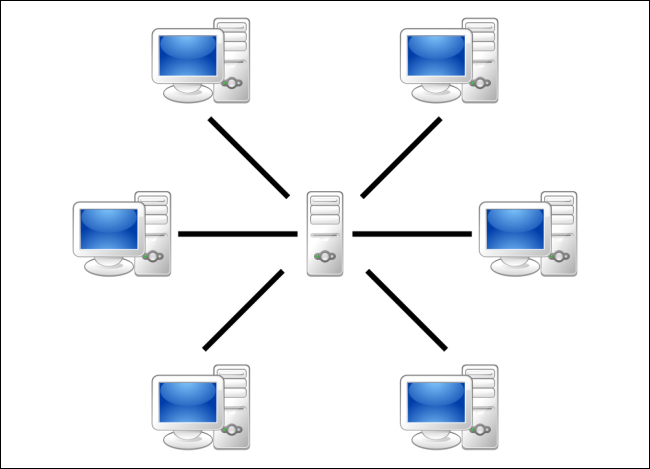
\includegraphics{centralserver.png}
De Centrale Bank kan fungeren als een zogenaamd tussenpersoon.
De Centrale Bank is verbonden met alle lokale banken.
Als een lokale bank informatie nodig heeft van een andere lokale bank,
kan hij de gegevens opvragen aan de centrale bank.
De centrale bank vervolgens vraagt aan de andere lokale bank.
En die stuurt de gegevens naar de centrale bank waardoor de centrale bank
de gegevens terug kan sturen de lokale bank die de gegevens had aangevraagd.\\

Elke lokale bank heeft een database waarin alle gegevens van hun klanten in staan.
Deze databases staan op een server van de lokale bank (dus een lokale server).

\section{Server Communicatie}


\subsection{Sockets}

\subsubsection{Java Applicatie}

\subsection{Message Protocols}

\subsubsection{MQ: Message Queuing}
Berichten worden door verschillende programmas gebruikt
om data met elkaar te delen tussen een zender en ontvanger.
Programmas gebruiken veel berichten na elkaar maar niet
alle berichtn kunnen tegelijk verwerkt worden.
Daarom is er een queue. Een gueue is een lijst met wachtende onderwerpen.
Message Queuing zorgt ervoor dat de messages in een volgorde verstuurd worden.

Message Queuing is een asynchroon communicatie protocol.
Dat houdt in dat het systeem een bericht in een queue lijst plaatst
en dat hoeft niet per direct verwerkt te worden.
Email is een voorbeeld van asynchroon communicatie.

Bij message queuing wordt er gebruik gemaakt van decoupling.
Dit is om de afzender en ontvanger te van elkaar te scheiden.
Decoupling is een proces dat delen van een systeem die afhankelijk
zijn van elkaar scheidt en zelfstandig maakt.

Message queuing werkt als volgt.
Een message producer(een applicatie bv) maakt een message aan met data erin.
De message stuurt hij dan naar een 'Message Broker'.
Een Message Broker houdt de message queue bij.
Wanneer de producer al zijn messages naar de message broker
gestuurd heeft stuurt de message broker de message queue naar
de message consumer.
De message consumer kan nu een voor een de messages in de message queue
verwerken en hoeft zo niet alle messages tegelijk te behandelen.
De messages hebben allemaal een topic.
Aan de hand van de topic reageren de message clients op de message queue die
door de message broker verstuurd wordt.


MQ brengt vele voordelen met zicht mee.
MQ heeft redundantie via persistentie om data te blijven behouden.
Je kan batches met messages zodat niet elke message appart wordt
verstuurd, maar dat je in 1 keer een aantal messages stuurt.
Dit zorgt voor de efficientie.
MQ kan ook in verschillende talen worden geschreven.
Berichten kunnen meerdere keren worden verstuurd.
Er kunnen ook meerdere message clients zijn per topic.

MQ heeft ook een aantal nadelen.
Bij MQ weet de message producer niet wie zijn clienten zijn.
Dus de message broker stuurt gewoon de message queue naar alle verbonden apparaten.
Een message client moet verbonden zijn om een bericht te kunnen ontvangen
anders wordt hij niet naar hem toegestuurd. \\

\paragraph{Toepasselijkheid op de Centrale Bank}
Op dit moment stuurt de client van de lokale bank berichten na mekaar steeds naar de lokale server.
Er is geen regeling of controle bij het sturen van de berichten.
Op kleine schaal is dat niet van belang.
Op een grotere schaal is komt dit wel in conflict met de efficientie van
de server connectie tussen de centrale bank en de lokale banken.
De centrale bank is verbonden met tientallen servers van de lokale banken.
De lokale banken sturen ook constant berichten naar de centrale bank.
De centrale bank kan dit niet in een keer verwerken.
Dus om dit probleem op te lossen maken we gebruik van MQ.
Message Queuing zorgt er voor dat de berichten(met queries voor de database)
die per client gestuurd worden naar de centrale bank eerst in een lijst worden gedaan
om in een keer gestuurd te worden naar de centrale bank.
Dit zorgt ook voor minder data belast.
De server kan dan gerust per queue de berichten een voor een verwerken.


\subsubsection{MQTT: Message Queuing Telemetry Transport}
MQ en MQTT hebben veel overeenkomsten maar zij verschillen toch van elkaar.
Hier is het de bedoeling dat de berichten naar een message client verstuurd worden,
i.p.v. meerdere message clients.
Dit protocol is heel licht.
Dus het is geen zwaar process dat veel resources neemt van de server en applicaties.
MQTT wordt vaak gebruikt bij IOT (Internet of Things).
Dus het is afhankeljk dat de apparaten met MQTT verbonden zijn binnen hetzelfde netwerk.

MQTT werkt op dezelfde manier als MQ.
Maar i.p.v. topics maakt MQTT gebruik van channels.
De message clients kunnen zich dan subscriben (inschrijven) bij zo een kanaal
om de berichten te ontvangen van een bepaald apparaat.
Dus gewoonlijk een message producer, message broker
en een message client.
Maar bij MQTT wordt de producer de publisher genoemd,
en de client wordt een subscriber genoemd.
Een publisher stuurt berichten en een subscriber ontvangt hen op een kanaal.
Een publish(bericht) kan je naar meerdere subscribers sturen.
MQTT heeft wel de mogelijkheid om een message queue te maken maar dat hoeft niet.

In MQTT is er een mogelijkheid om QoS (Quality of Service) te hebben.
Hiermee kan er aangegeven worden welke berichten belangrijk zijn,
en welke weer niet.
QoS bestaat uit 3 niveaus:
\begin{description}
	\item [QoS-0 (niveau 1):] Het bericht wordt een aantal keer verstuurd en niet opgeslagen.
		Er wordt ook niet gecontroleerd of het bericht aankomt.
	\item [QoS-1 (niveau 2):] De publisher stuurt een bericht tenminste 1 keer en verwacht
		een response van de broker als conformatie dat de broker het bericht naar alle
		subscribers gestuurd heeft.
	\item [QoS-2 (niveau 3):] De publisher stuurt maar 1 bericht naar de broker. De broker
		bevestigd aan de publisher dat het bericht is ontvangen.
		Daarna stuurt de publisher een bevestiging terug dat hij de bevestiging van de broker
		ontvangen heeft. 
\end{description}
MQTT is niet veilig omdat de gegevens gewoon als plain text verstuurd worden.

\paragraph{Toepasselijkheid op de Centrale Bank}
MQTT kan gebruikt worden bij het sturen van de queries naar de centrale bank.

\section{Advies}
%Wat advieseer je aan de mensen om te doen bij het maken van de bank?


\section{Kwaliteitseisen}
%Welke kwaliteitseisen zijn er gesteld voor je de centrale bank en hoe pak je ze aan?


\subsection{Security}

\paragraph{Encryptie}
Als we het hebben over encryptie,
dan hebben wij het gewoon over het versleutelen van data.
SSL en Hashing zijn hier goede voorbeelden van.
Hashing is een 

\paragraph{Firewall}
\paragraph{Arduino beveiliging}

\subsection{Effectiviteit}




\end{document}
